% ============================================================================
% TimeSlackDestroy Operator — Illustration
% ============================================================================
% Compile with: pdflatex or xelatex
% Required packages: tikz, amsmath, amssymb
% ============================================================================

\documentclass[border=10pt,tikz]{standalone}
\usepackage[utf8]{inputenc}
\usepackage{amsmath,amssymb}
\usepackage{tikz}
\usetikzlibrary{arrows.meta, positioning, decorations.pathmorphing,
                calc, backgrounds, fit, shapes.geometric,
                patterns, fadings}

% ── Color Palette ──
\definecolor{depot}{HTML}{2C3E50}
\definecolor{custHigh}{HTML}{E74C3C}    % High liberation score
\definecolor{custMed}{HTML}{F39C12}     % Medium liberation score
\definecolor{custLow}{HTML}{27AE60}     % Low liberation score (lots of slack)
\definecolor{station}{HTML}{3498DB}
\definecolor{routeLine}{HTML}{7F8C8D}
\definecolor{fwdArrow}{HTML}{2980B9}
\definecolor{bwdArrow}{HTML}{8E44AD}
\definecolor{slackFill}{HTML}{D5F5E3}
\definecolor{lockFill}{HTML}{FADBD8}
\definecolor{selectionBg}{HTML}{FEF9E7}
\definecolor{annotColor}{HTML}{6C3483}
\definecolor{bgGray}{HTML}{F8F9FA}

\begin{document}
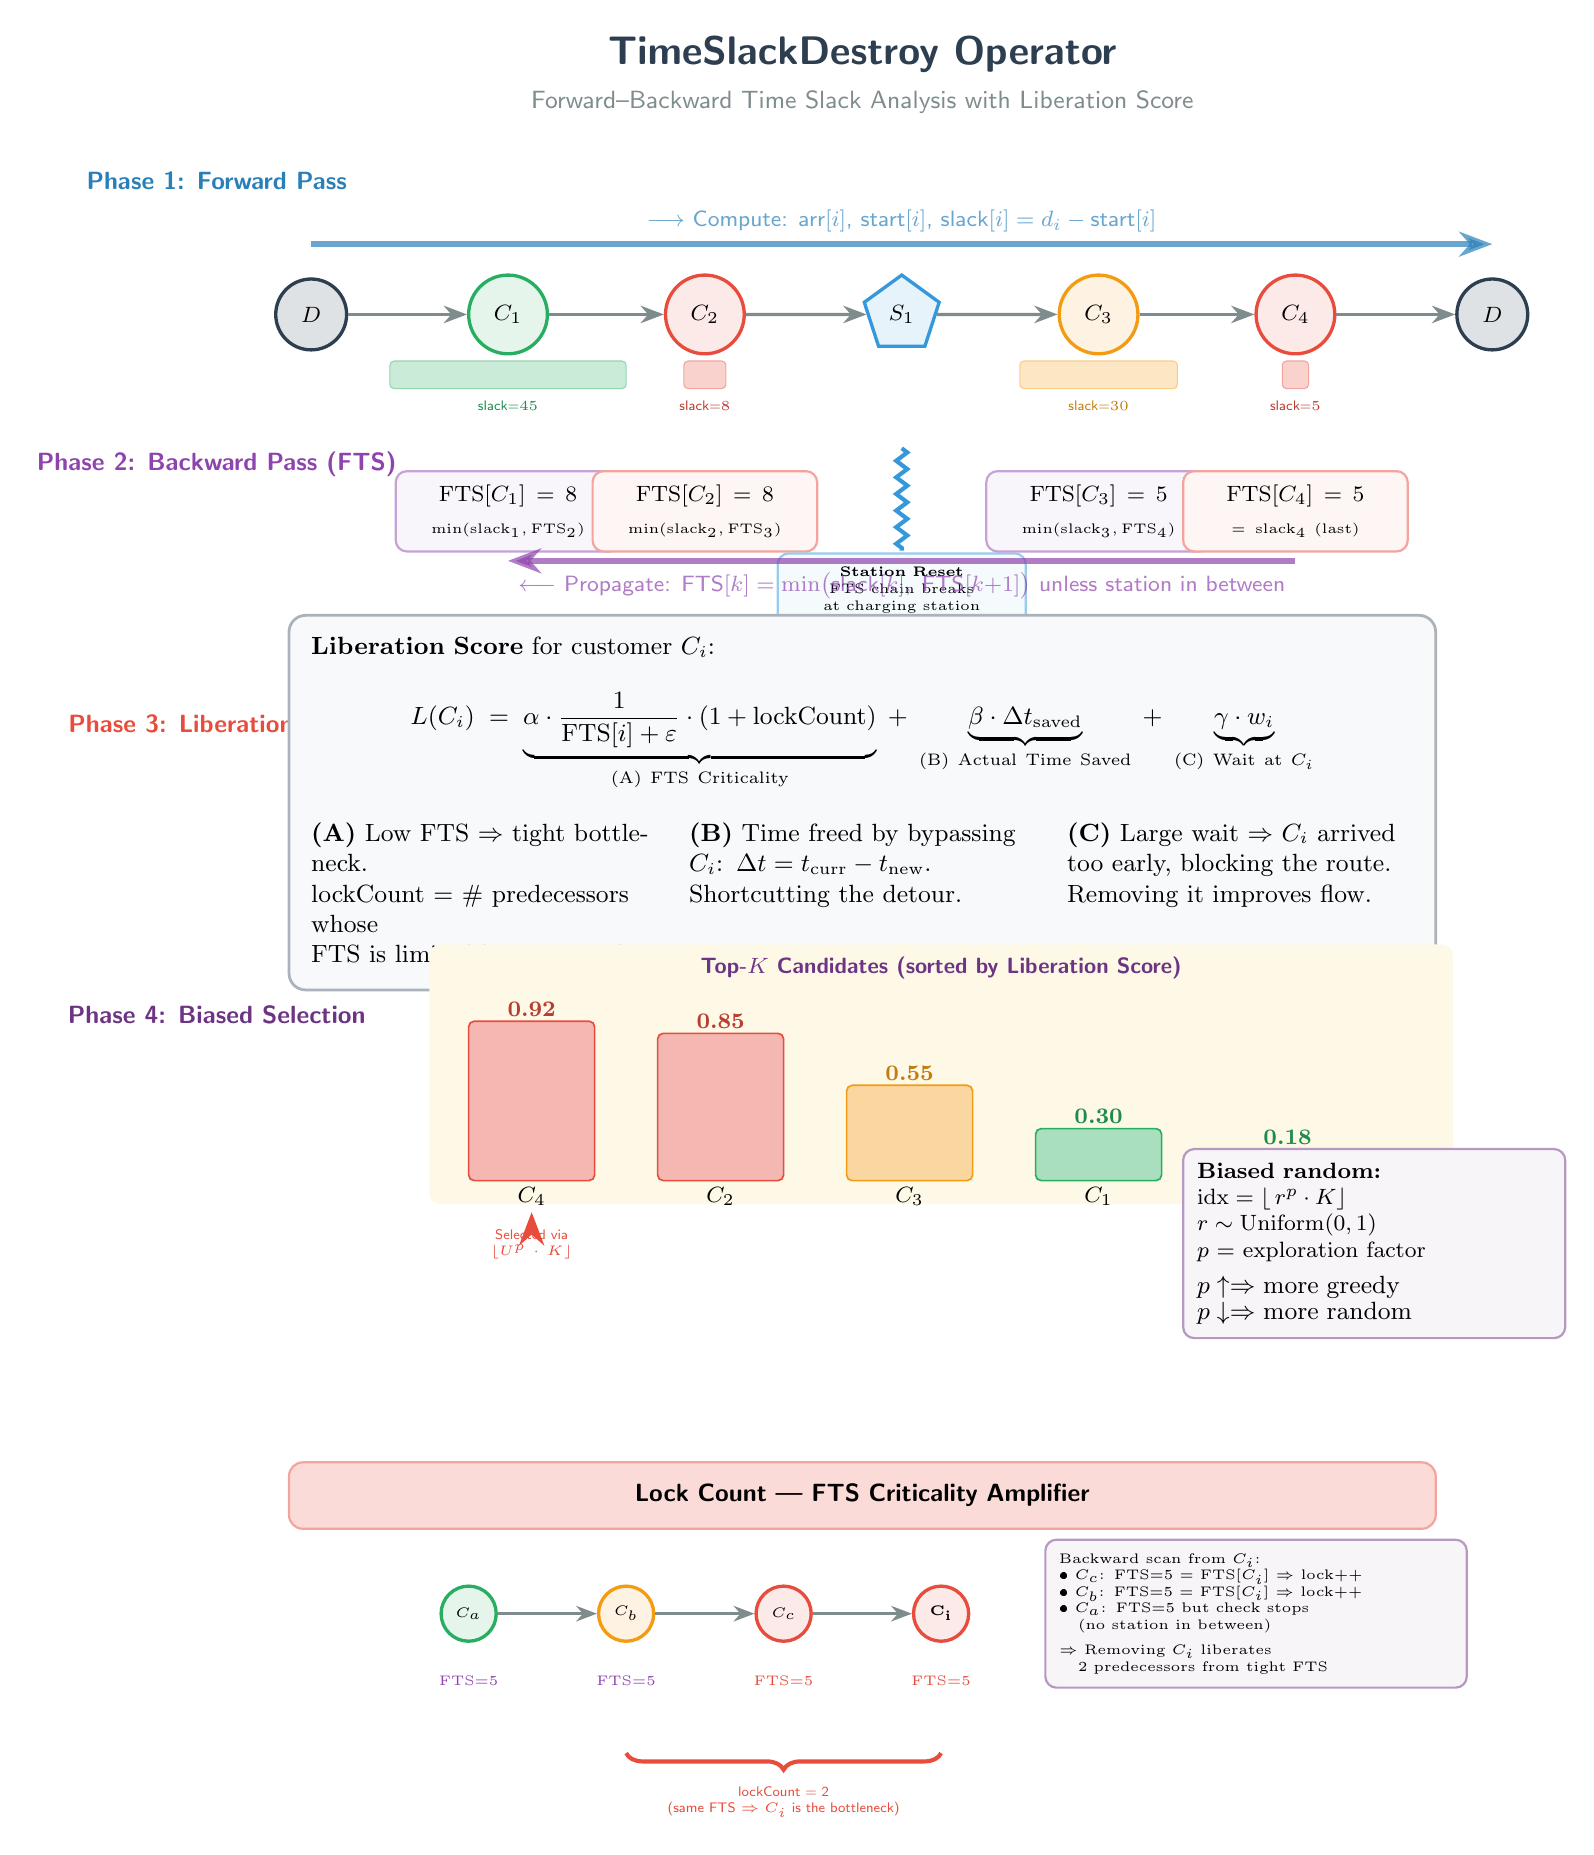
\begin{tikzpicture}[
    >=Stealth,
    node distance=1.8cm,
    every node/.style={font=\small},
    depot node/.style={
        circle, draw=depot, fill=depot!15, line width=1.2pt,
        minimum size=9mm, font=\footnotesize\bfseries
    },
    cust node/.style={
        circle, draw=#1, fill=#1!12, line width=1.2pt,
        minimum size=10mm, font=\footnotesize\bfseries
    },
    station node/.style={
        regular polygon, regular polygon sides=5,
        draw=station, fill=station!12, line width=1.2pt,
        minimum size=10mm, font=\footnotesize\bfseries
    },
    slack bar/.style={
        draw=none, fill=slackFill, rounded corners=1pt
    },
    lock indicator/.style={
        draw=custHigh!60, fill=lockFill, rounded corners=2pt,
        line width=0.8pt, dashed
    },
    phase label/.style={
        font=\small\bfseries\sffamily, text=#1
    },
    info box/.style={
        draw=#1!50, fill=#1!5, rounded corners=4pt,
        line width=0.8pt, inner sep=5pt, font=\footnotesize
    },
]

% ════════════════════════════════════════════════════════════════════
% TITLE
% ════════════════════════════════════════════════════════════════════
\node[font=\Large\bfseries\sffamily, text=depot] at (7, 9.8)
    {TimeSlackDestroy Operator};
\node[font=\small\sffamily, text=routeLine] at (7, 9.2)
    {Forward--Backward Time Slack Analysis with Liberation Score};

% ════════════════════════════════════════════════════════════════════
% PART A: ROUTE WITH TIMING DATA (Forward Pass)
% ════════════════════════════════════════════════════════════════════

\node[phase label=fwdArrow] at (-1.2, 8.2) {Phase 1: Forward Pass};

% Route nodes
\node[depot node] (d0) at (0, 6.5) {$D$};
\node[cust node=custLow] (c1) at (2.5, 6.5) {$C_1$};
\node[cust node=custHigh] (c2) at (5, 6.5) {$C_2$};
\node[station node] (s1) at (7.5, 6.5) {$S_1$};
\node[cust node=custMed] (c3) at (10, 6.5) {$C_3$};
\node[cust node=custHigh] (c4) at (12.5, 6.5) {$C_4$};
\node[depot node] (d1) at (15, 6.5) {$D$};

% Route edges
\foreach \a/\b in {d0/c1, c1/c2, c2/s1, s1/c3, c3/c4, c4/d1} {
    \draw[->, routeLine, line width=1.2pt] (\a) -- (\b);
}

% Forward pass arrows (above)
\draw[->, fwdArrow, line width=2pt, opacity=0.7]
    ([yshift=12pt]d0.north) -- ([yshift=12pt]d1.north)
    node[midway, above, font=\footnotesize\sffamily, text=fwdArrow]
    {$\longrightarrow$ Compute: $\text{arr}[i]$, $\text{start}[i]$, $\text{slack}[i] = d_i - \text{start}[i]$};

% Slack bars below each customer
\foreach \nd/\sval/\col in {c1/45/custLow, c2/8/custHigh, c3/30/custMed, c4/5/custHigh} {
    \pgfmathsetmacro{\bw}{\sval/15}  % Scale bar width
    \draw[fill=\col!25, draw=\col!50, rounded corners=1.5pt]
        ([xshift=-0.5*\bw cm, yshift=-2pt]\nd.south)
        rectangle +(\bw cm, -0.35cm);
    \node[below=0.45cm of \nd, font=\tiny\sffamily, text=\col!80!black]
        {slack=$\sval$};
}

% ════════════════════════════════════════════════════════════════════
% PART B: BACKWARD PASS (FTS with Station-Aware Reset)
% ════════════════════════════════════════════════════════════════════

\node[phase label=bwdArrow] at (-1.2, 4.6) {Phase 2: Backward Pass (FTS)};

% FTS values
\node[info box=bwdArrow, text width=2.5cm, align=center] (fts1) at (2.5, 4.0)
    {$\text{FTS}[C_1] = 8$\\[2pt]\tiny $\min(\text{slack}_1, \text{FTS}_2)$};
\node[info box=custHigh, text width=2.5cm, align=center] (fts2) at (5, 4.0)
    {$\text{FTS}[C_2] = 8$\\[2pt]\tiny $\min(\text{slack}_2, \text{FTS}_3)$};

% Station reset annotation
\draw[station, line width=1.5pt, decorate,
      decoration={zigzag, amplitude=2pt, segment length=6pt}]
    (7.5, 4.8) -- (7.5, 3.5);
\node[info box=station, text width=2.8cm, align=center, font=\tiny] at (7.5, 3.0)
    {\textbf{Station Reset}\\FTS chain breaks\\at charging station};

\node[info box=bwdArrow, text width=2.5cm, align=center] (fts3) at (10, 4.0)
    {$\text{FTS}[C_3] = 5$\\[2pt]\tiny $\min(\text{slack}_3, \text{FTS}_4)$};
\node[info box=custHigh, text width=2.5cm, align=center] (fts4) at (12.5, 4.0)
    {$\text{FTS}[C_4] = 5$\\[2pt]\tiny $= \text{slack}_4$ (last)};

% Backward arrows
\draw[<-, bwdArrow, line width=2pt, opacity=0.7]
    ([yshift=-3pt]fts1.south) -- ([yshift=-3pt]fts4.south |- fts1.south)
    node[midway, below, font=\footnotesize\sffamily, text=bwdArrow]
    {$\longleftarrow$ Propagate: $\text{FTS}[k] = \min\bigl(\text{slack}[k],\;\text{FTS}[k{+}1]\bigr)$ unless station in between};

% ════════════════════════════════════════════════════════════════════
% PART C: LIBERATION SCORE COMPUTATION
% ════════════════════════════════════════════════════════════════════

\node[phase label=custHigh] at (-1.2, 1.3) {Phase 3: Liberation Score};

% Formula box
\node[draw=depot!40, fill=bgGray, rounded corners=6pt, line width=1pt,
      inner sep=8pt, text width=14cm, align=left, font=\small]
      (formula) at (7, 0.3) {
    \textbf{Liberation Score} for customer $C_i$:
    \vspace{3pt}
    \[
    L(C_i) \;=\;
    \underbrace{\alpha \cdot \frac{1}{\text{FTS}[i] + \varepsilon}
                \cdot (1 + \text{lockCount})}_{\text{(A) FTS Criticality}}
    \;+\;
    \underbrace{\beta \cdot \Delta t_{\text{saved}}}_{\text{(B) Actual Time Saved}}
    \;+\;
    \underbrace{\gamma \cdot w_i}_{\text{(C) Wait at } C_i}
    \]

    \vspace{2pt}
    \begin{minipage}[t]{4.4cm}
        \textbf{(A)} Low FTS $\Rightarrow$ tight bottleneck.\\
        lockCount = \# predecessors whose\\
        FTS is limited by same node.
    \end{minipage}
    \hfill
    \begin{minipage}[t]{4.4cm}
        \textbf{(B)} Time freed by bypassing\\
        $C_i$: $\Delta t = t_{\text{curr}} - t_{\text{new}}$.\\
        Shortcutting the detour.
    \end{minipage}
    \hfill
    \begin{minipage}[t]{4.4cm}
        \textbf{(C)} Large wait $\Rightarrow$ $C_i$ arrived\\
        too early, blocking the route.\\
        Removing it improves flow.
    \end{minipage}
};

% ════════════════════════════════════════════════════════════════════
% PART D: SELECTION MECHANISM (Roulette with Top-K)
% ════════════════════════════════════════════════════════════════════

\node[phase label=annotColor] at (-1.2, -2.4) {Phase 4: Biased Selection};

% Bar chart for scores
\begin{scope}[shift={(2, -4.5)}]
    % Background
    \fill[selectionBg, rounded corners=4pt] (-0.5, -0.3) rectangle (12.5, 3.0);
    \node[font=\footnotesize\sffamily\bfseries, text=annotColor] at (6, 2.7)
        {Top-$K$ Candidates (sorted by Liberation Score)};

    % Bars
    \foreach \i/\lbl/\val/\col in {
        0/$C_4$/0.92/custHigh,
        1/$C_2$/0.85/custHigh,
        2/$C_3$/0.55/custMed,
        3/$C_1$/0.30/custLow,
        4/$C_5$/0.18/custLow%
    } {
        \pgfmathsetmacro{\bh}{\val * 2.2}
        \fill[\col!40, draw=\col, rounded corners=2pt, line width=0.6pt]
            (\i*2.4, 0) rectangle ++(1.6, \bh);
        \node[font=\footnotesize\bfseries, text=\col!80!black]
            at (\i*2.4 + 0.8, \bh + 0.15) {\val};
        \node[font=\footnotesize\sffamily] at (\i*2.4 + 0.8, -0.2) {\lbl};
    }

    % Selection arrow
    \draw[->, custHigh, line width=2pt]
        (0.8, -0.6) -- (0.8, -0.4)
        node[below=2pt, font=\tiny\sffamily, text=custHigh, text width=2cm, align=center]
        {Selected via\\$\lfloor U^p \cdot K \rfloor$};

    % Annotation: exploration factor
    \node[info box=annotColor, text width=4.5cm, align=left] at (11.5, -0.8) {
        \textbf{Biased random:}\\
        $\text{idx} = \lfloor \,r^p \cdot K \rfloor$\\
        $r \sim \text{Uniform}(0,1)$\\
        $p$ = exploration factor\\[2pt]
        \small $p \uparrow \Rightarrow$ more greedy\\
        \small $p \downarrow \Rightarrow$ more random
    };
\end{scope}

% ════════════════════════════════════════════════════════════════════
% PART E: LOCK COUNT DETAIL (Inset)
% ════════════════════════════════════════════════════════════════════

\begin{scope}[shift={(0, -8.5)}]
    % Lock count illustration
    \node[draw=custHigh!50, fill=lockFill, rounded corners=5pt,
          line width=0.8pt, inner sep=8pt, text width=14cm] (lockbox) at (7, 0) {
        \begin{minipage}{\textwidth}
        \centering
        \textbf{\sffamily Lock Count — FTS Criticality Amplifier}
        \end{minipage}
    };

    % Mini route showing lock propagation
    \node[cust node=custLow, minimum size=7mm, font=\tiny\bfseries] (lc1) at (2, -1.5) {$C_a$};
    \node[cust node=custMed, minimum size=7mm, font=\tiny\bfseries] (lc2) at (4, -1.5) {$C_b$};
    \node[cust node=custHigh, minimum size=7mm, font=\tiny\bfseries] (lc3) at (6, -1.5) {$C_c$};
    \node[cust node=custHigh, minimum size=7mm, font=\tiny\bfseries] (lc4) at (8, -1.5) {$\mathbf{C_i}$};

    \foreach \a/\b in {lc1/lc2, lc2/lc3, lc3/lc4} {
        \draw[->, routeLine, line width=1pt] (\a) -- (\b);
    }

    % FTS annotations
    \node[below=3mm of lc1, font=\tiny, text=bwdArrow] {FTS=5};
    \node[below=3mm of lc2, font=\tiny, text=bwdArrow] {FTS=5};
    \node[below=3mm of lc3, font=\tiny, text=custHigh] {FTS=5};
    \node[below=3mm of lc4, font=\tiny, text=custHigh] {FTS=5};

    % Lock chain bracket
    \draw[custHigh, line width=1.5pt, decorate,
          decoration={brace, amplitude=6pt, mirror}]
        ([yshift=-14mm]lc2.south) -- ([yshift=-14mm]lc4.south)
        node[midway, below=8pt, font=\tiny\sffamily, text=custHigh, text width=4cm, align=center]
        {lockCount = 2\\(same FTS $\Rightarrow$ $C_i$ is the bottleneck)};

    % Explanation
    \node[info box=annotColor, text width=5cm, align=left, font=\tiny] at (12, -1.5) {
        Backward scan from $C_i$:\\
        \textbullet\ $C_c$: FTS=5 = FTS[$C_i$] $\Rightarrow$ lock++\\
        \textbullet\ $C_b$: FTS=5 = FTS[$C_i$] $\Rightarrow$ lock++\\
        \textbullet\ $C_a$: FTS=5 but check stops\\
        \quad (no station in between)\\[3pt]
        $\Rightarrow$ Removing $C_i$ liberates\\
        \quad 2 predecessors from tight FTS
    };
\end{scope}

\end{tikzpicture}
\end{document}
